\chapter{Тестирование и анализ результатов} \label{ch6}
В данной главе будет рассмотрено тестирование сервера и клиента визуализатора. Так как сервис разработан в учебных целях, тестирование производится вручную за счет анализа методов, написанных на Java для каждой модели. Тестирование сервера производится с помощью утилиты Postman.
\section{Тестирование сервера} \label{ch6:sec1}
Тестирование сервера производилось с помощью утилиты Postman. В нашем случае будет есть одна основная точка доступа, на вход которой подаётся исходный код на языке Java, а в качестве ответа ожидается JSON, в котором содержится структура AST в двух видах – в облегчённом (simple) и в расширенном (extended). На рис. 6.1 изображен соответствующий POST-запрос.

\begin{figure}[h]
	\center
	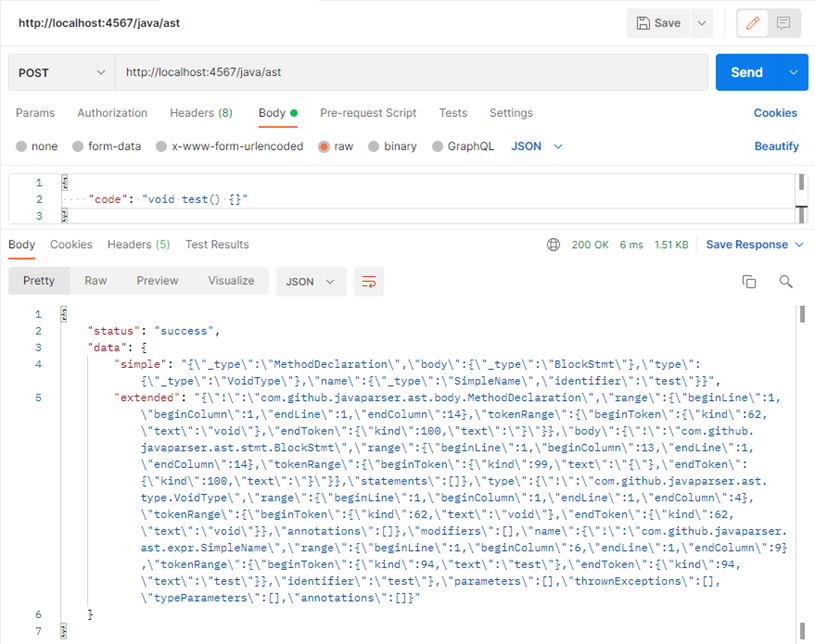
\includegraphics [scale=0.65] {my_folder/images/my/20}
	\caption{Тестирование сервера визуализатора} 
	\label{fig:20}  
\end{figure}

В запросе мы подаем на вход исходный код, который требуется парсить, а на выходе получаем результат работы JavaParser в двух видах: simple (который потребуется для рисования) и extended (с указанием связей с исходным кодом и прочей информацией). Исходя из результата тестирования можно сделать вывод, что сервер работает так, как надо.
\section{Тестирование клиента} \label{ch6:sec2}
Тестирование клиента проводится вручную в таких браузерах, как Яндекс Браузер, Google Chrome, Firefox, Opera, Edge за счет анализа ряда методов, написанных на Java для каждой модели. Ниже приведены рисунки с результатом работы визуализатора для одного из методов (sumOdd, упомянутый в первой главе) в каждом браузере.

\begin{figure}[h]
	\center
	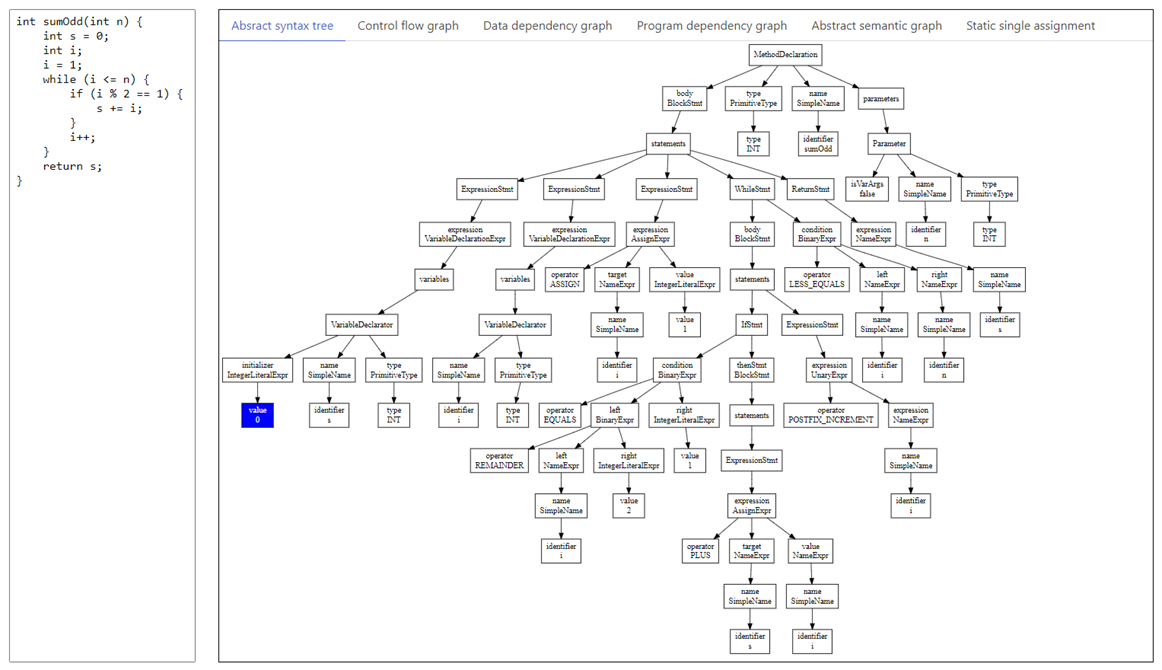
\includegraphics [scale=0.5] {my_folder/images/my/21}
	\caption{Построенное AST в браузере Edge}
	\label{fig:21}
\end{figure}

Как можно увидеть на рис. 6.2, в дереве присутствуют только семантически значимые узлы. Если блок подсвечен синим цветом, то это означает, что все его наследники скрыты. Интерфейс визуализатора реализован в соответствии со схематичным представлением, представленным ранее.

\begin{figure}[h]
	\center
	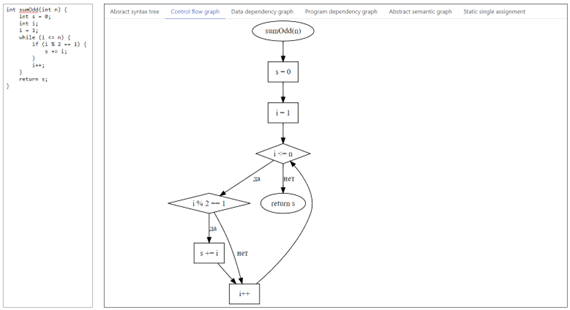
\includegraphics [scale=0.6] {my_folder/images/my/22}
	\caption{Построенный CFG в Яндекс браузере}
	\label{fig:22}
\end{figure}
\newpage
На рис. 6.3 видно, что в построенном CFG используются стандартные формы для обозначения узлов: эллипс для обозначения начала или конца, прямоугольник для обычных операторов, ромб для узлов принятия решений. Рёбра, выходящие из узлов принятия решений, имеют обозначения, дающие понять, по какому ребру переходить в случае, если условие истинно, а по какому в случае, если ложно.

\begin{figure}[h]
	\center
	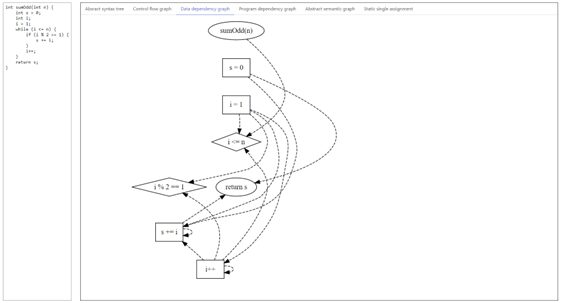
\includegraphics [scale=0.48] {my_folder/images/my/23}
	\caption{Построенный DDG в браузере Chrome}
	\label{fig:23}
\end{figure}
На рис. 6.4 изображен DDG, полностью совпадающий с примером визуализации из первой главы. Узлы размещаются так же, как и в CFG, с помощью этого будет проще понять её устройство.
\begin{figure}[h]
	\center
	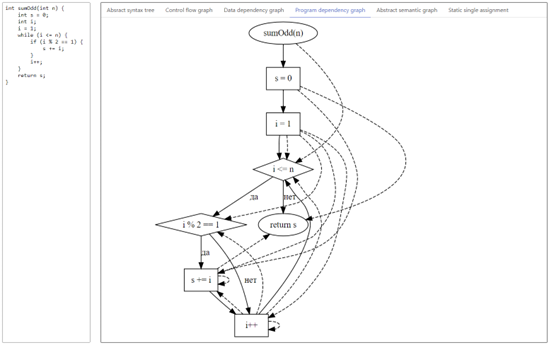
\includegraphics [scale=0.65] {my_folder/images/my/24}
	\caption{Построенный PDG в браузере Opera}
	\label{fig:24}
\end{figure}
\newpage
На рис. 6.5 изображен PDG, также полностью совпадающий с примером визуализации из первой главы. Модель так же строится на основе CFG, но дополняется ребрами из DDG.
\begin{figure}[h]
	\center
	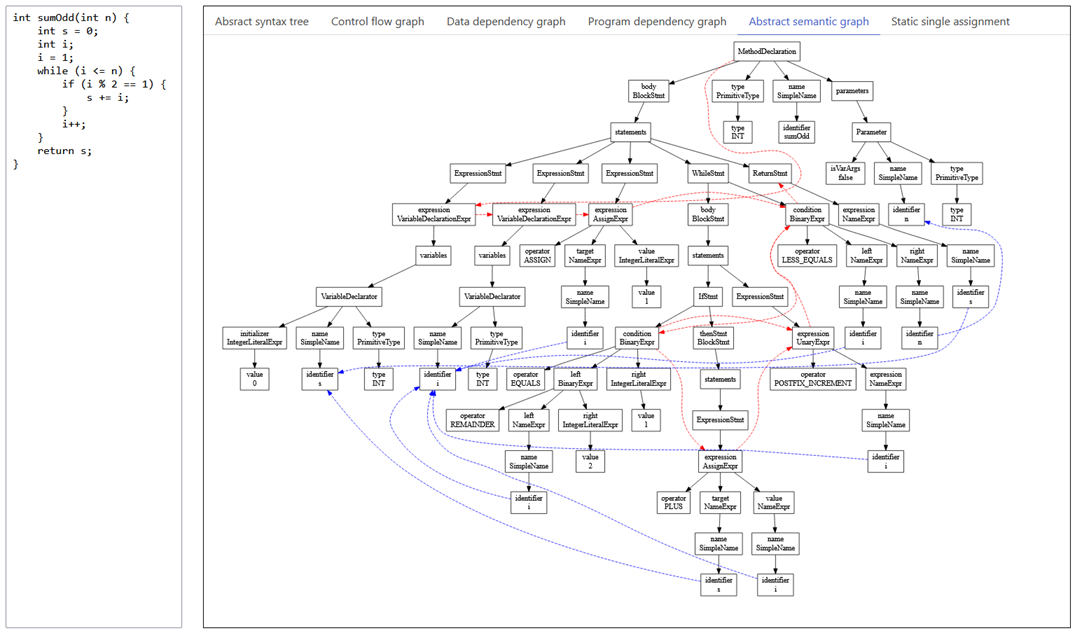
\includegraphics [scale=0.55] {my_folder/images/my/25}
	\caption{Построенный ASG в браузере Firefox}
	\label{fig:25}
\end{figure}

На рис. 6.6 видно, что при отрисовке ребра между соседними инструкциями для наглядности обозначаются красными пунктирными стрелками, а рёбра между объявлениями и использованием переменных пунктирными синими.

\begin{figure}[h]
	\center
	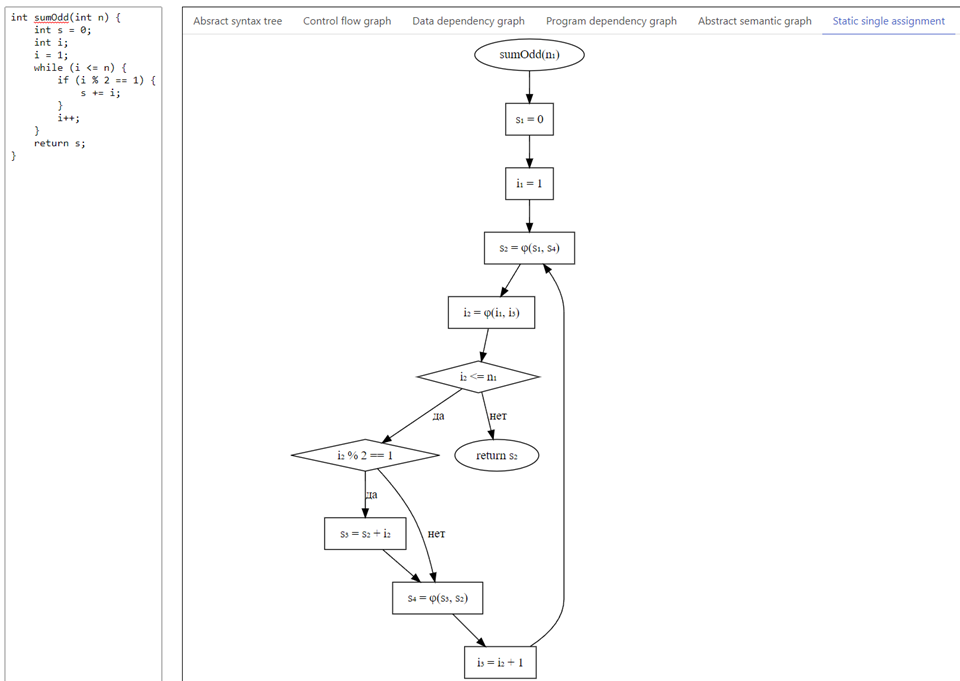
\includegraphics [scale=0.5] {my_folder/images/my/26}
	\caption{Построенное SSA в Яндекс браузере}
	\label{fig:26}
\end{figure}

На рис. 6.7 видно, что SSA строится правильно. Также хочется отметить, что клиент корректно работает во всех браузерах, используемых при тестировании.

\begin{figure}[h]
	\center
	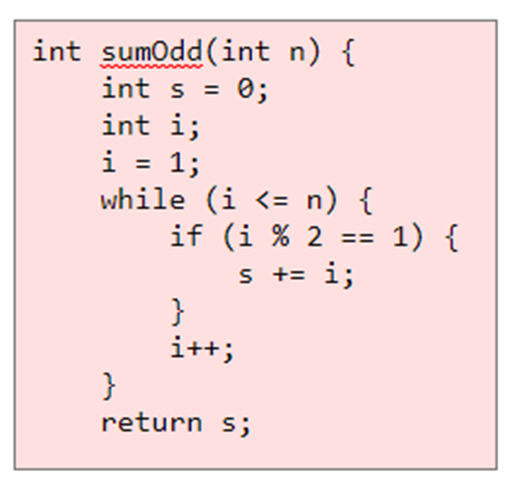
\includegraphics [scale=0.5] {my_folder/images/my/27}
	\caption{Неправильно введенный код}
	\label{fig:27}
\end{figure}

На рис. 6.8 можно увидеть, что если код написан неверно, то интерфейс подсвечивается красным цветом и отрисовка и изменение уже нарисованной модели не происходит.
\section{Выводы по главе} \label{ch6:sec3}
В данной главе рассмотрено тестирование сервера и клиента визуализатора. Сервер протестирован с помощью утилиты Postman, а клиент тестировался в разных браузерах для разных методов, написанных на Java. В отчете приведен один из них. Все модели строятся правильно и интерфейс работает так, как было задумано. Из результатов тестирования можно сделать вывод, что сервис выполняет поставленные задачи.
\newpage